\chapter{Analysis and Discussion}
\label{analysis}

\section{Patterns}
\subsection{Detection}
There are more than 100,000 times more similar sequences found in the
scale/filter coefficients than in the wavelet/shift coefficients. The large
difference in number of sequences found between the two types of coefficients
is due to the fact that the LOC metric is a cumulative metric. The typical
trend of a LOC signal is growth. This makes finding similar sequences using
shift coefficients (i.e., along the time axis) less likely.

\paragraph{}
No patterns were detected in shift coefficients. This can be explained by the
fact that the 16 similar sequences in shift coefficients are not similar within
the same group of sequences.

Additionally, the shift coefficients are incomparable to the filter coefficients
because they were found in a fundamentally different way of signal
transformation. Mixing both types of coefficients would neglect the way the
coefficients were found and invalidate the patterns comprising sequences of
both types of coefficients.

\subsection{Similarity}
The patterns that were detected show strong similarity among signals. The
similarity was demonstrated in Figure \ref{figure:patterns_plots} in section
\ref{section:seqs_patterns}. The figure presents an arbitrary pattern and its
occurrences across different projects. The figure also demonstrates how wavelet
transforms 'smooths out' differences in details by scaling and filtering the
signals.

\paragraph{}
One of the properties of the Haar function is that it is reversible. This
means that it is possible to pick any wavelet on any level of decomposition
that resulted from Haar transform and use it to re-compose the original signal.
This is a useful property for testing a pattern. Figure
\ref{figure:type_a_pattern} shows the type A pattern \#3256 projected onto the
original signals of two projects.

\begin{figure}[H]
\caption{Type A pattern \#3256 in two projects}\label{figure:type_a_pattern}
\centering
	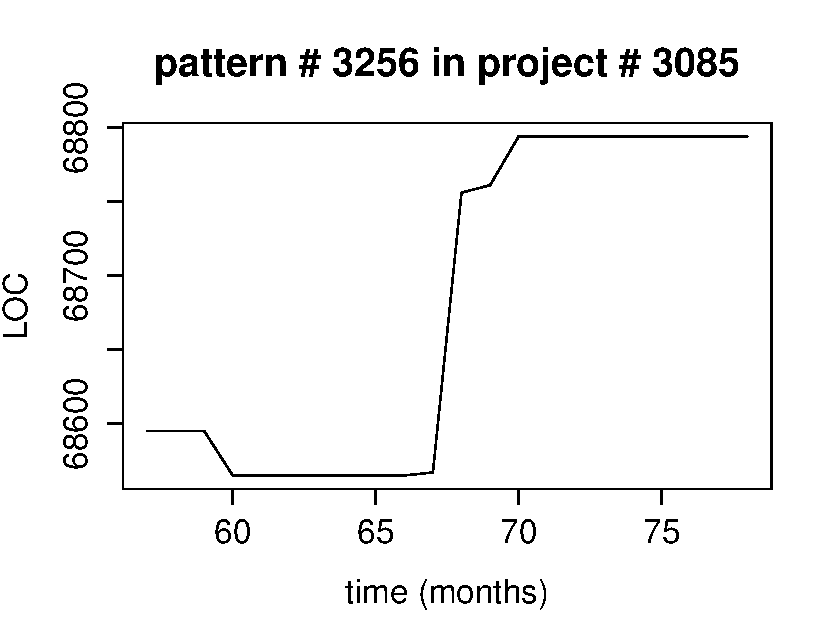
\includegraphics[width=196pt]{images/pattern_a_3085.pdf}
	\hspace{1em}
	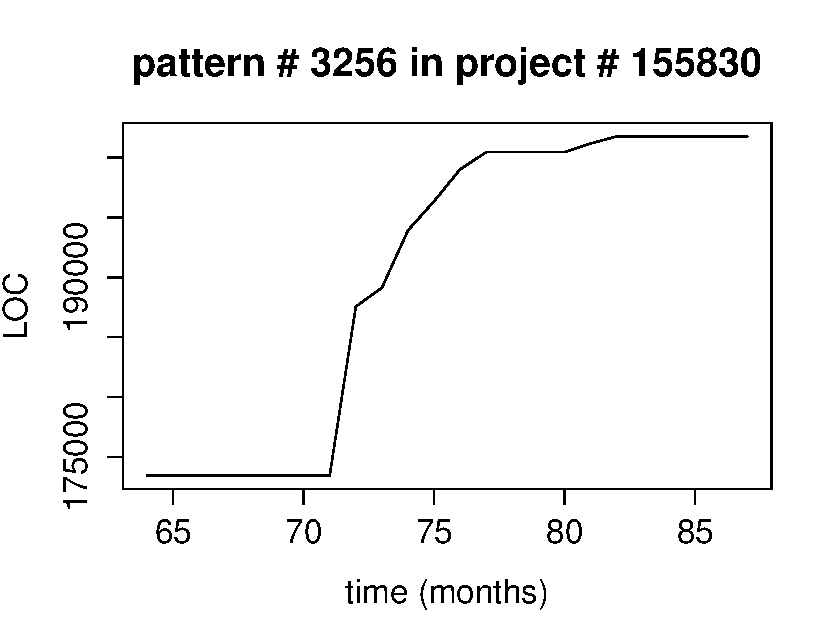
\includegraphics[width=196pt]{images/pattern_a_155830.pdf}
\end{figure}

\indent
Figure \ref{figure:type_a_pattern} shows the wavelets of the occurrence of type
A pattern \#3256 in two dead projects. The pattern starts near, and lasts until
the end of code evolution of the projects. This figure shows that the pattern
ends in a stagnation of LOC change. The shapes of both wavelets are similar,
even though the wavelets are not scaled in this figure -- project \#3085 is
about 30\% smaller than project \#155830 when comparing the LOC values.

\subsection{Warning signs}
The classification of the patterns detected in dead projects (see section
\ref{section:patterns_dead}) was needed to distinguish possible warning signs
from other recurring events. The type A patterns were expected to be the best
candidates for representing warning signs because of the property that they
last until the end of code evolution of a dead project.

\paragraph{}
Type B patterns are the patterns not lasting until the end of code evolution of
dead projects. The typical shape of the type B patterns found in LOC signals in
this study are sub-linear growth in LOC. The other two common shapes of type B
patterns is an almost super-linear growth sine shape and super-linear decay.
The latter shows a free fall in LOC. Figure \ref{figure:type_b_pattern}
illustrates all three shapes.

\begin{figure}[H]
\caption{Typical type B patterns}\label{figure:type_b_pattern}
\caption*{\footnotesize\textit{\\[1em](left) Sub-linear growth\\(center)
Super-linear/sine-shaped growth\\(right) Super-linear decay}\\[1em]}
\centering
	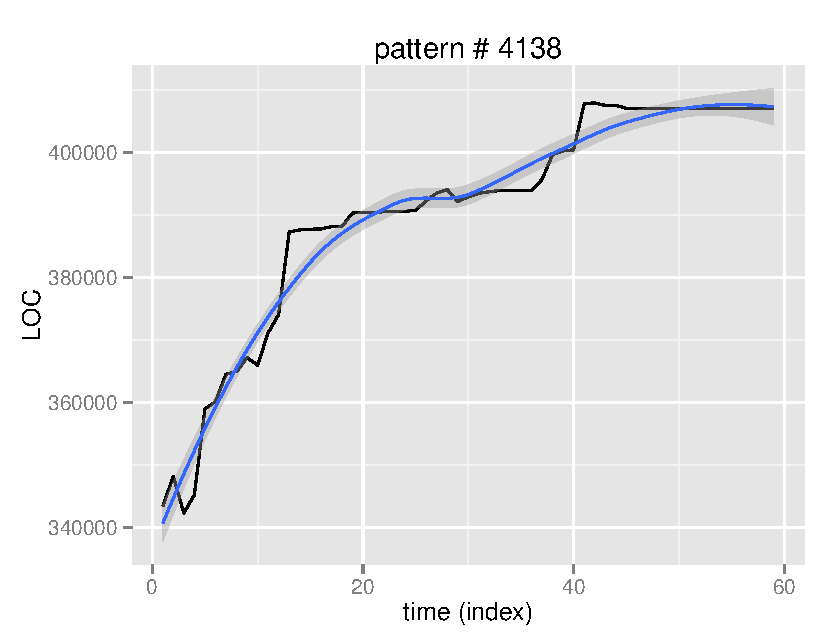
\includegraphics[width=128pt]{images/pattern_b_sub.pdf}
	\hspace{1em}
	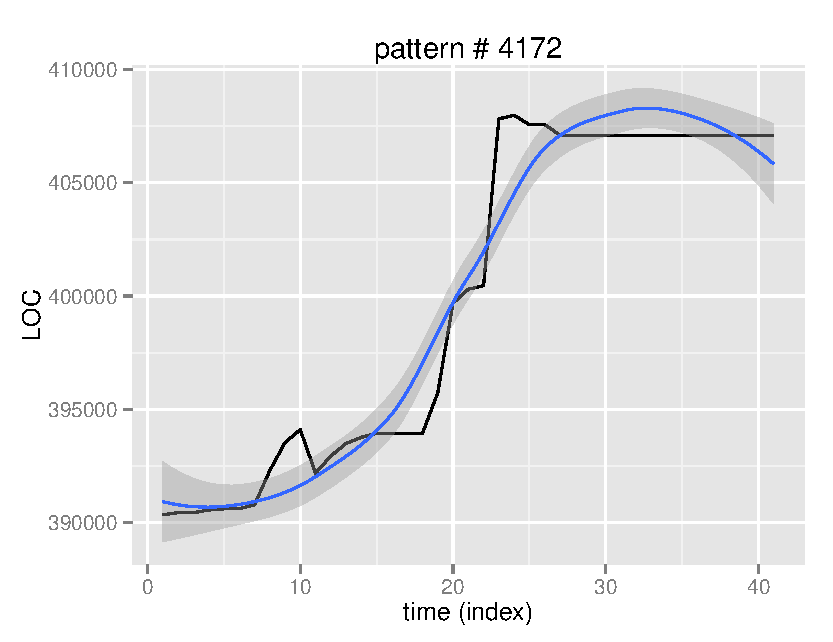
\includegraphics[width=128pt]{images/pattern_b_sine.pdf}
	\hspace{1em}
	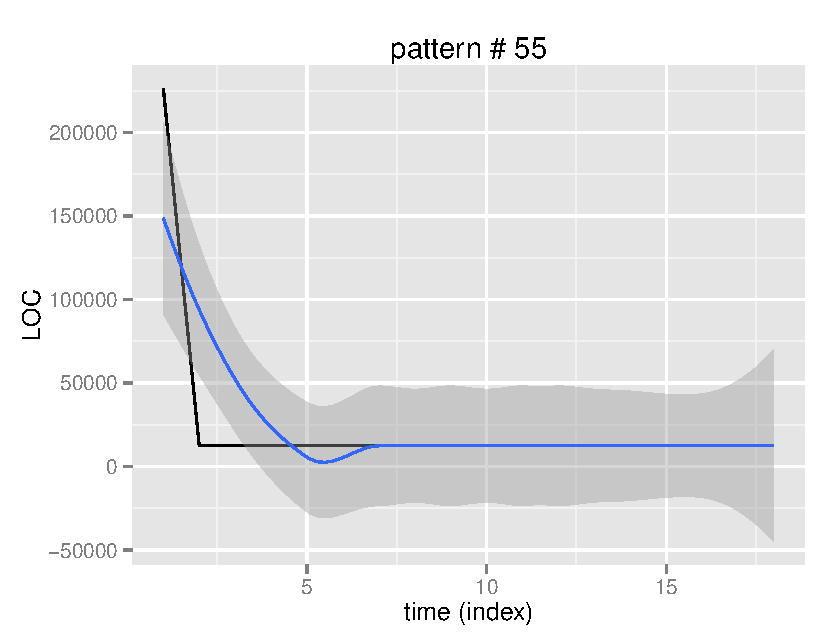
\includegraphics[width=128pt]{images/pattern_b_super.pdf}
\end{figure}

\noindent
Occurrences of type AB patterns are found anywhere in the evolution of dead
projects. This means that they may or may not be a candidate for representing a
warning sign. The difficulty is the fact that the AB patterns do not occur in a
consistent manner: in one project it may be an indicator for end of code
evolution, while in another project it does not.

\subsubsection{False-negatives}
When looking back at the projects selected for survival analysis in group G0
(section \ref{section:group_g0}), 4 out of 93 projects \textit{not} having a
type A pattern died. The patterns indicating the impending end of code
evolution were not detected as such. However, all 4 projects had occurrences of
type AB patterns.

\subsubsection{False-positives}
Taking the projects in group G1 (section \ref{section:group_g1}), 79 out of 93
projects were still alive by April 2014. The alive projects already lived
longer since diagnosis than the dead projects in the same group. This means
that not all patterns of type A can be interpreted as a warning sign.

\paragraph{}
It can be a possibility to treat AB patterns also as possible warning signs,
because of the property that in \textit{some} projects the pattern occurs near,
and lasts until the end of code evolution. This, however, will yield more
false-positive results because a pattern occurring anywhere in a project's
evolution could hardly be an indicator of the end of that evolution.
On the other hand, treating the AB patterns explicitly \textit{not} as possible
warning signs -- as in this study -- will yield more false-negative results.

\section{Survival analysis}
\label{section:kp_survival}
The Kaplan-Meier estimation of the survival function of the projects as shown
in Figure \ref{figure:kp_survival} suggests that projects in group G1 -- the
projects having an occurrence of a type A pattern -- die earlier than the
projects in group G0 -- the projects without an occurrence of a type A pattern.

\paragraph{}


\begin{comment}
More about:
- How come G1 have higher survival chances in the first year?
- How come G1 and G0 have equal chances between 3.2 and 3.8 years?
\end{comment}

\begin{comment}
- Analyse results
- Conclude and interpret results
- Answer hypotheses and research questions
- Threats to validity
- Discussion
- Future work
 
This chapter contains the analysis and interpretation of the results. The
research questions are answered as best as possible given the results that were
obtained. The analysis also discussed parts of the questions that were left
unanswered.

An important topic is the validity of the results.
What methods of validation were used?
Could the results be generalized to other cases?
What threats to validity can be identified?

There is room here to discuss the results of related scientific literature here
as well.
How do the results obtained here relate to other work, and what consequences are
there?
Did your approach work better or worse?
Did you learn anything new compared to the already existing body of knowledge?
Finally, what could you say in hindsight on the research approach by followed?
What could have done better?
What lessons have been learned?
What could other researchers use from your experience?

A separate section should be devoted to ‘future work,’ i.e., possible extension
points of your work that you have identified. Other researchers (or yourself)
could use those as a starting point.

Refer to Chapters 3.7 and 4 in this example thesis at Paul’s
homepage\footnote{http://homepages.cwi.nl/~paulk/thesesMasterSoftwareEngineering/2006/ReneWiegers.pdf}.
\end{comment}
